\problemname{FiboFish}

\begin{wrapfigure}{r}{5.5cm}
    \centering
    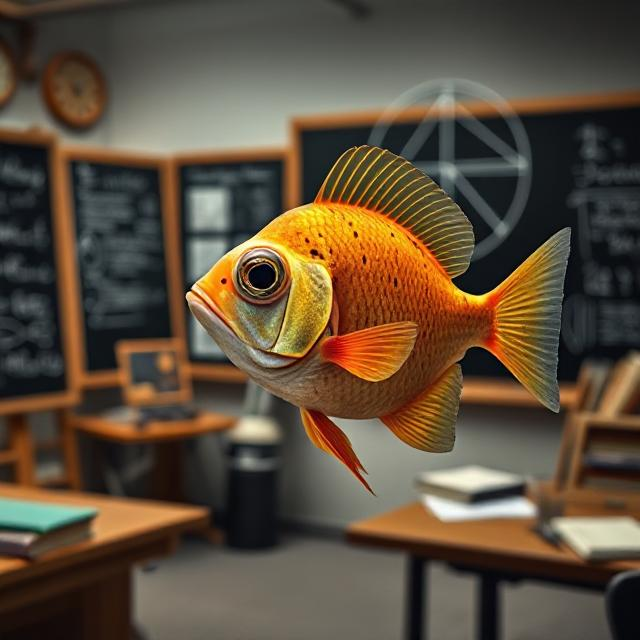
\includegraphics[width=5.5cm]{Fibofish.jpeg}
\end{wrapfigure}
% Source: deepai.org

Le professeur Léonard Fibonacci, grand amateur de poissons exotiques, a récemment découvert une étrange espèce de poissons mathématiciens qui communiquent uniquement avec des nombres codés. Cette espèce, nommée \textbf{KARWA} (Kryptic Algorithmic Researchers of the Watery Abyss), encode ses messages en utilisant la \textit{suite de Fibonacci}. Votre rôle est d'aider le professeur à comprendre ce codage afin de rendre le langage poisson compréhensible.

La suite de Fibonacci est définie comme suit : en posant $F_1 = 1$, $F_2 = 2$\footnote{Le professeur déteste commencer par $0$, cela lui rappelle trop le binaire. C'est pour cela que l'indexation des termes de la suite commence bien à $1$ pour $F_1 = 1$ !}, on a la récurrence $F_n = F_{n-1} + F_{n-2}$ pour tout $n \geq 3$.

Étant donné un nombre entier $N$, votre tâche sera de donner le codage $C$ de $N$. Pour ce faire, il faut représenter $N$ comme la somme de nombres distincts de la suite de Fibonacci et additionner leur indices en choisissant une décomposition qui minimise la somme des indices des termes de Fibonacci utilisés. Par exemple, si $N = 14$, on obtient $C = 7$ car
\begin{itemize}
    \item $14 = 13 + 1 = F_6 + F_1$, ce qui donne $7$ comme candidat,
    \item $14 = 8 + 3 + 2 + 1 = F_5 + F_3 + F_2 + F_1$, ce qui donne $11$, et $7$ est inférieur à $11$.
\end{itemize}

\begin{Input}
    L'entrée consiste en une unique ligne contenant un entier $N$ ($1 \leq N \leq 10^{18}$).
\end{Input}

\begin{Output}
    Un entier $C$, le codage de $N$.
\end{Output}
